\chapter{Problema del corpo nero}

\section{Richiami su energia trasportata da onde}
\begin{definition}[Intensit\`a]
L'\textbf{intensit\`a} di un'onda \`e data da
\[I=\frac{dE}{dA_\perp dt}\qquad\qquad [I]=\frac{\mathrm{W}}{\mathrm{m}^{2}}.\]
La \textbf{radianza} \`e l'intensit\`a per angolo solido
\[I_\Omega=\frac{dE}{dA_\perp dtd\Omega}=\dd \Omega I.\]
\end{definition}

\begin{definition}[Emittanza e Irradianza]
L'\textbf{emittanza} come la potenza emessa da una supeficie per unit\`a di superficie. Si indica con $M$.\\
L'\textbf{irradianza} \`e la potenza ricevuta su una superficie per unit\`a di superficie. Anche questa si indica con $I$.
\end{definition}

\section{Pressione di radiazione}
Consideriamo un'onda elettromagnetica che incide su una superficie conduttrice in modo ortogonale. Sia $\sigma$ la densit\`a di carica superficiale. Se la superficie ha area $A$ allora possiamo scrivere la forza di Lorentz come
\[\frac{\vec F}A=\sigma(\vec E+\vec v\times \vec B).\]
L'onda induce un movimento delle cariche interno alla superficie e $\vec v\times \vec B$ ha verso sempre diretto verso la superficie

\begin{figure}[!htb]
    \centering
    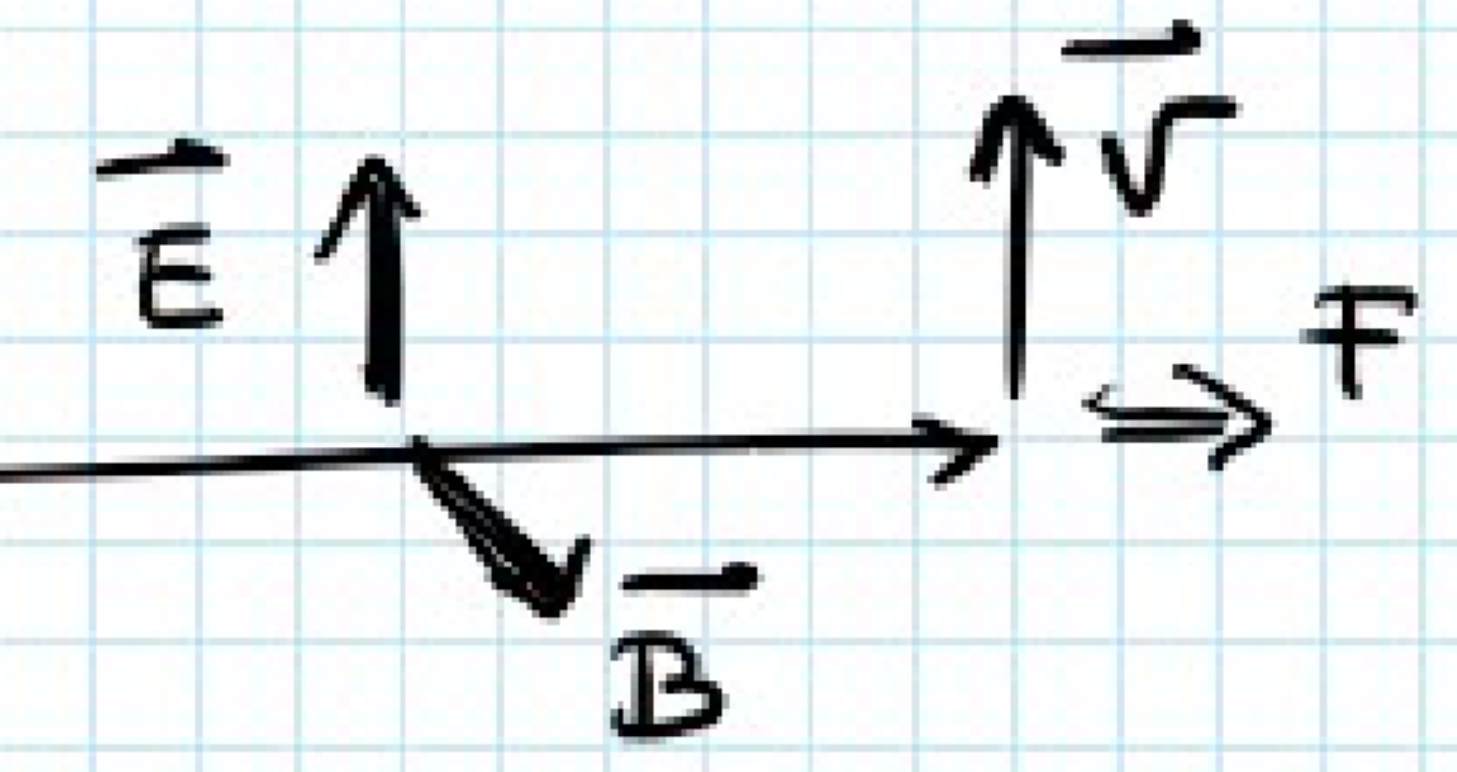
\includegraphics[width=5cm]{images/onda_elettromagnetica_che_incide_ortogonalmente.png}
\end{figure}

\noindent
Calcoliamo l'intensit\`a assorbita\footnote{potenza per area} e la pressione esercitata sulla superficie
\[\begin{cases}
~\\
I_{\text{assorbita}}=\dfrac{\vec F\cdot \vec v}A=\sigma \vec E\cdot \vec v+\cancelto{0}{\sigma \vec v\cdot(\vec v\times \vec B)}=\sigma \vec E\cdot \vec v\\\\
p\overset{\vec E\text{ parallelo}}{\overset{\text{a superficie}}=}\sigma\abs{\vec v\times \vec B}=\sigma vB=\sigma v\dfrac Ec=\dfrac{I_{\text{assorbita}}}c\\~
\end{cases}\]
Se la superficie assorbe tutta l'energia che riceve
\begin{align*}
&\Delta E=I_{\text{assorbita}}\Delta t A\\
&\abs{\vec p}=\frac1cI_{\text{assorbita}}\Delta t A
\end{align*}
Se la superficie riflette tutta l'energia che riceve
\begin{align*}
&\Delta E=0\\
&\abs{\vec p}=2\frac1cI_{\text{assorbita}}\Delta t A
\end{align*}

\subsection{Gas di onde elettromagnetiche}
Consideriamo una semisfera dentro la quale ci sono onde elettromagnetiche distribuite in modo omogeneo e isotropo. Sia $w$ la densit\`a di energia nella semisfera (ben definita per omogeneit\`a).\\
Consideriamo poi una superficie $A$ come in figura perfettamente assorbente e cerchiamo di capire quanta energia e quantit\`a di moto riceve per unit\`a di tempo.

\begin{figure}[!htb]
    \centering
    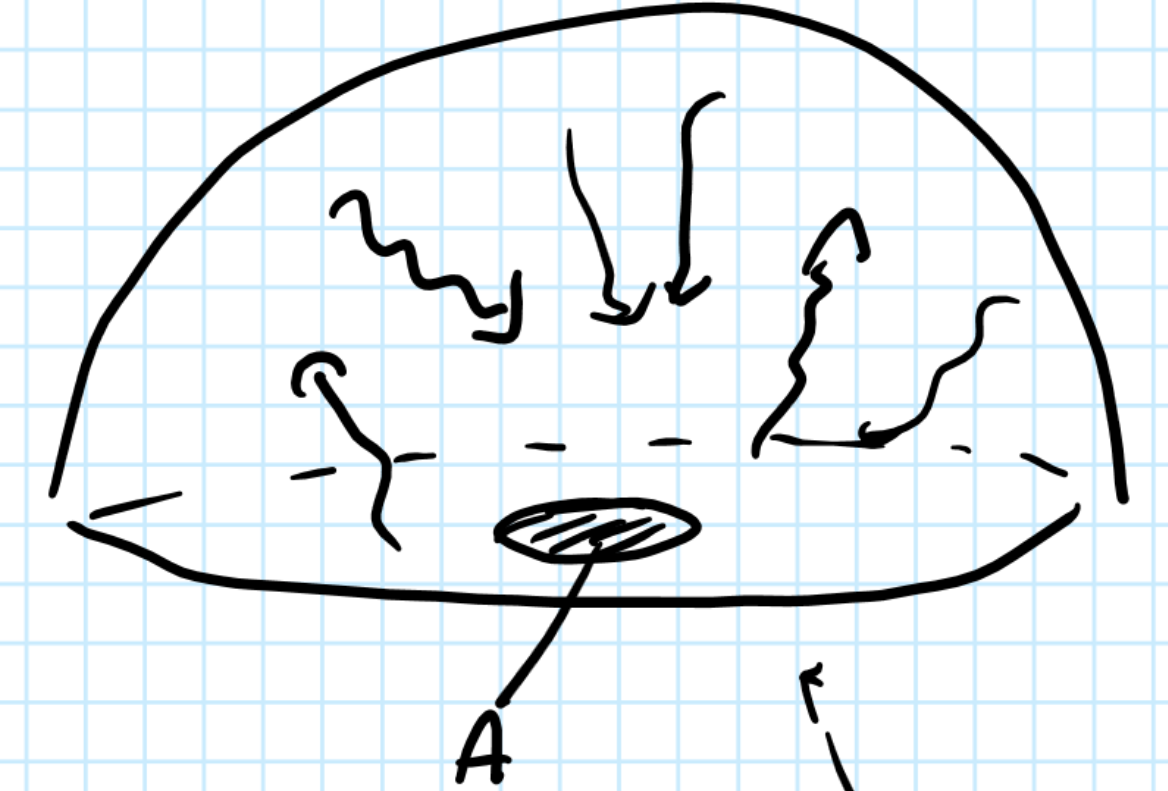
\includegraphics[width=5cm]{images/semisfera_luce.png}
\end{figure}

\noindent
Consideriamo un ragionamento analogo a quello fatto per il modello dei gas perfetti:\\
Fissata una direzione consideriamo il cilindro di particelle che si scontrano contro la nostra area in una unit\`a di tempo $dt$

\begin{figure}[!htb]
    \centering
    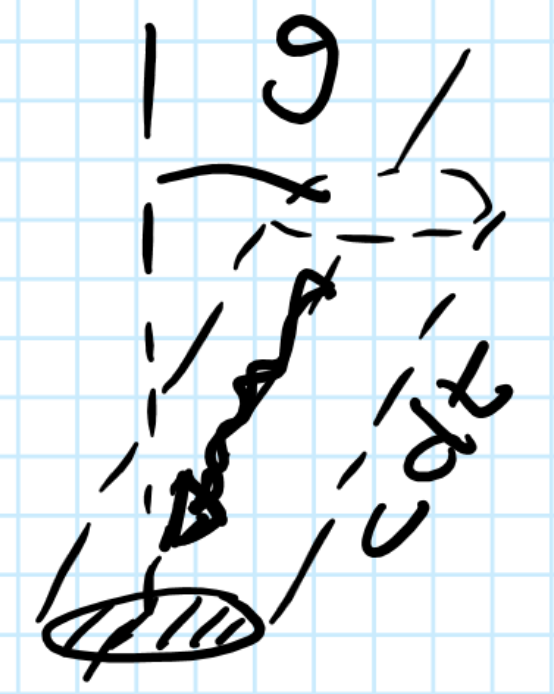
\includegraphics[width=2.5cm]{images/cilindretto_luce.png}
\end{figure}

\noindent
Il volume del cilindretto \`e $A cdt\cos \theta$, dunque l'energia che colpisce $A$ \`e
\[w Acdt\cos \theta.\]
Segue che tutta l'energia che raggiunge $A$ in un intervallo di tempo $dt$ \`e l'integrale sull'angolo solido diviso per due\footnote{stiamo considerando solo met\`a sfera} della quantit\`a trovata, cio\`e
\[dE=\frac12\int_\Omega w Acdt\cos\theta \frac{d\Omega}{4\pi}=\frac12\frac{w Acdt}{4\pi}\int_\Omega\cos\theta 2\pi \under{=d(\cos\theta)}{\sin\theta d\theta} =\frac{w cAdt}4,\]
dunque $I_{\text{assorbita}}=\dfrac{w c}4$.
\medskip

\noindent
Consideriamo ora l'impulso assorbito
\[d\abs{\vec p_\perp}\pasgnlmath={m_{\mathrm{luce}}=0}\frac{dE}c\cos\theta=\frac12\int_\Omega \frac w c Acdt(\cos\theta)^2 \frac{d\Omega}{4\pi}=\frac{w Adt}6,\]
dunque la pressione \`e
\[p=\frac w6.\]

\bigskip

\noindent
Se la superficie \`e riflettente allora $I_{\text{assorbita}}=0$ per definizione, quindi
\[d\abs{\vec p_\perp}=2\frac{w Adt}6\implies p=\frac w3.\]

\section{Radiazione di Corpo nero}
\subsection{Definizione e corpo nero scatola}
\begin{definition}[Assorbanza]
Un corpo irraggiato assorbe una frazione $a(\nu)$ della radiazione a frequenza $\nu$ che riceve. Questa quantit\`a \`e detta \textbf{assorbanza} (relativa alla frequenza $\nu$).
\end{definition}

\begin{definition}[Corpo bianco e corpo nero]
Se $a(\nu)=0$ per ogni $\nu$ allora il corpo \`e detto \textbf{bianco} o \textbf{perfettamente riflettente}.\\
Se $a(\nu)=1$ per ogni $\nu$ allora il corpo \`e detto \textbf{nero} o \textbf{perfettamente assorbente}.
\end{definition}

\begin{remark}
Poich\'e ogni oggetto contiene qualche particella carica, ogni corpo irraggia delle onde elettromagnetiche.
\end{remark}


\noindent
Una possibile realizzazione di un corpo nero \`e una scatola con pareti opache e un forellino minuscolo come in figura

\begin{figure}[!htb]
    \centering
    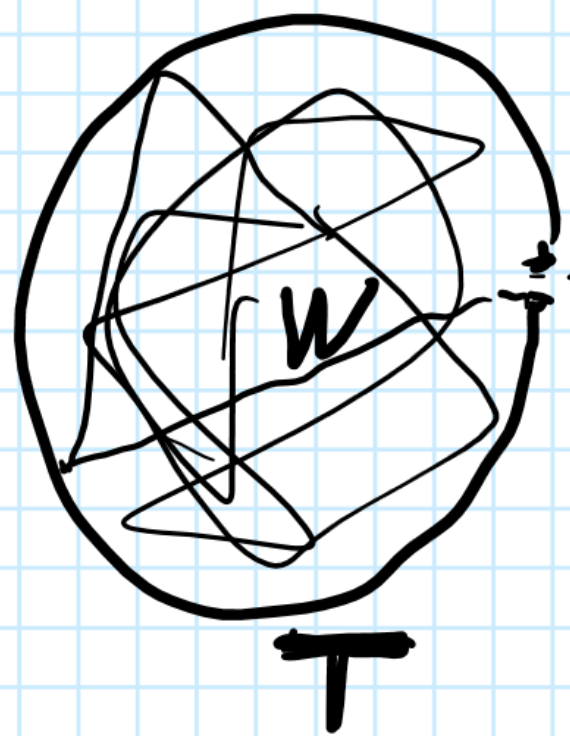
\includegraphics[width=2.5cm]{images/corpo_nero_scatola.png}
\end{figure}

\begin{proposition}
La densit\`a di energia di un corpo nero dipende solo da $T$. Inoltre la densit\`a di energia per ogni frequenza dipende solo da $T$.
\end{proposition}
\begin{proof}
Supponiamo di avere due corpi neri scatola, una con pareti interne perfettamente riflettenti e piene di energia e l'altra con pareti interne perfettamente assorbenti e poca energia.

\begin{figure}[!htb]
    \centering
    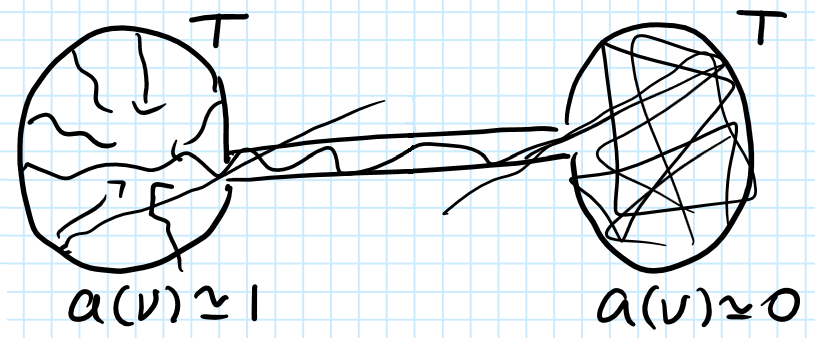
\includegraphics[width=7cm]{images/dimostrazione_w_dipende_solo_da_T.png}
\end{figure}

\noindent
Mettendo a contatto i forellini come in figura notiamo che le onde passerebbero dalla scatola riflettente a quella assorbente. Questo significa che anche se le sorgenti hanno la stessa temperatura, una tenderebbe a scaldarsi, negando il secondo principio.
\bigskip

\noindent
Se ora immaginiamo di mettere nel corridoio tra le scatole una parete che fa passare solo luce di una certa frequenza negeremmo di nuovo i principi della termodinamica se le densit\`a di energia fossero diverse per frequenze diverse.
\end{proof}

\subsection{Legge di Kirchhoff}
In questa sezione $I$ \`e la potenza dell'onda, non l'irradianza. L'irradianza \`e $a(\nu)I_\nu$ per una ogni frequenza.

\noindent
Immaginiamo ora di inserire un secondo corpo nero dentro la scatola. 
Per mantenere la sola dipendenza da $T$ si ha che per il corpo nero interno $I=M$, cio\`e assorbe tanta energia quanta ne emette.\\
Definiamo questa quantit\`a \textbf{radiazione di corpo nero}.

\begin{figure}[!htb]
    \centering
    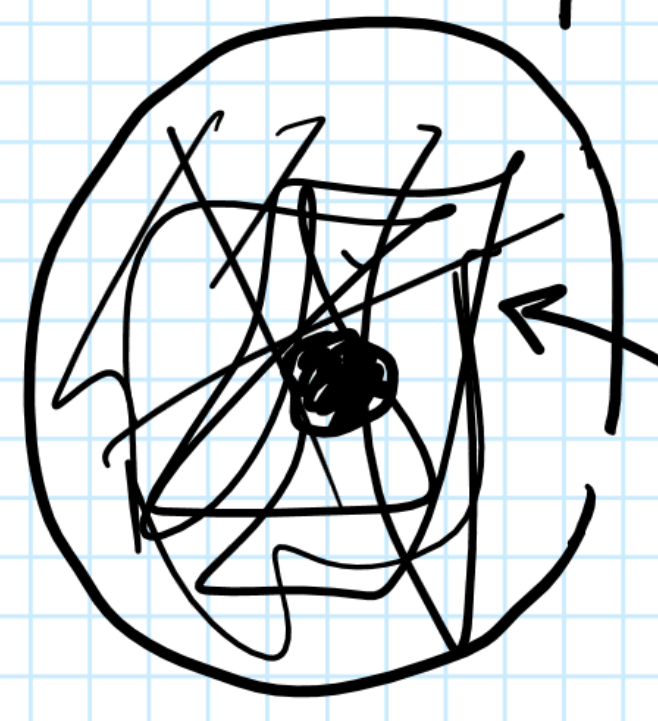
\includegraphics[width=2.5cm]{images/corpo_nero_con_dentro_corpo_nero.png}
\end{figure}

\noindent
Consideriamo ora lo steso scenario ma con un corpo non nero. Con un argomento analogo $aI=M$ in generale e per ogni frequenza $a(\nu)I_\nu=M_\nu$.

\begin{figure}[!htb]
    \centering
    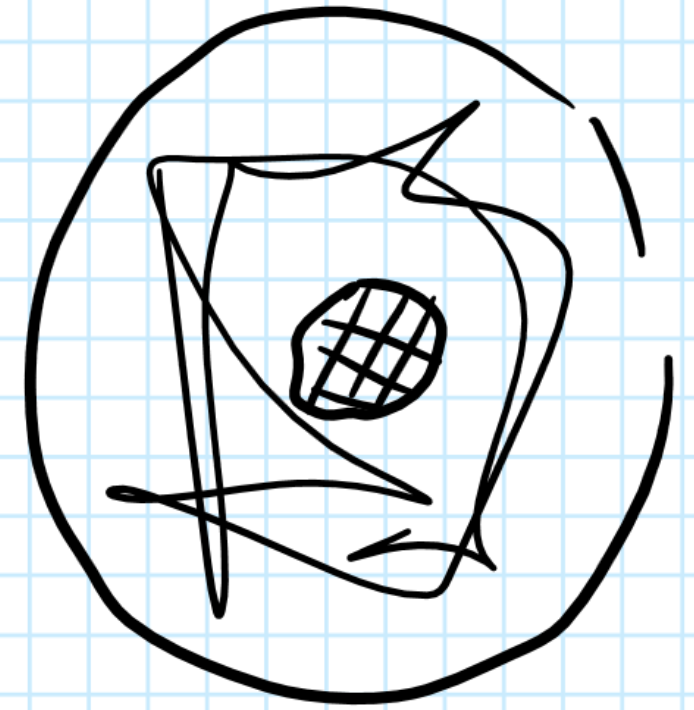
\includegraphics[width=2.5cm]{images/corpo_nero_con_dentro_corpo_grigio.png}
\end{figure}

\begin{remark}[Legge di Kirchhoff]
Il rapporto tra quanta radiazione un corpo emette rispetto ad un corpo nero alla stessa temperatura \`e esattamente la frazione di energia che assorbe
\[\frac{M}{M_{\text{corpo nero}}}=a.\]
Questa \`e la \textbf{legge di Kirchhoff}.
\end{remark}

\noindent Il ragionamento fatto funziona anche per frequenze fissate, quindi
\[\frac{M_\nu}{a(\nu)}=(M_\nu)_{\text{corpo nero}}.\]
Questo dimostra che la radiazione di corpo nero $(M_\nu)_{\text{corpo nero}}$ \`e una legge universale.

\subsection{Legge di Stefan-Boltzmann}
In questa sezione $I_\nu$ indica l'irradianza, quindi ci\`o che avevamo denotato con $a(\nu)I_\nu$ nella sezione precedente.

\noindent
Osserviamo che
\[M=\int_0^\infty I_\nu d\nu=\frac{E_{\text{totale emessa}}}{\Delta t A}.\]
Sperimentalmente Stefan scopre che
\[M\propto T^4.\]
Boltzmann deduce questo risultato per via teorica:

\begin{theorem}[Legge di Stefan-Boltzmann]\label{LeggeStefanBoltzmann}
Vale la \textbf{legge di Stefan-Boltzmann}
\[M=\sigma T^4.\]
\end{theorem}
\begin{proof}
Modelliamo il corpo nero come una scatola con pareti interne perfettamente riflettenti.\\
Per definizione $w=\frac UV$, inoltre questo rapporto dipende solo da $T$.\\ Abbiamo calcolato prima che per pareti perfettamente riflettenti $p=\frac w3$, che dipende solo da $T$. Ricordando che per sistemi idrostatici $dU=TdS-pdV$, si ha che
\[dS=\frac {dU}T+\frac pTdV=\frac VTdw+\pa{\frac wT+\frac pT}dV.\]
Poich\'e $w$ dipende solo da $T$, se $T$ \`e costante allora $w$ \`e costante, quindi dalla relazione sopra segue che
\[s\doteqdot\ppb VST=\ppb VSw=\pa{\frac wT+\frac pT}=\frac 43 \frac wT,\]
dunque $S=sV$ e $s$ dipende solo da $T$.\\
Sviluppando di nuovo il primo principio si ha
\[wdV+Vdw=dU=TdS-pdV=TdS-\frac w3dV=T(sdV+Vds)-\frac w3dV.\]
Dividendo per $V$ troviamo
\[dw=Tds+\pa{Ts-\frac 43w}\frac{dV}V.\]
Portando $Tds$ al primo membro osserviamo che,
poich\'e $w$ e $s$ dipendono solo da $T$ (e in particolare non da $V$) entrambi i membri sono nulli, 
\[dw=Tds\quad\text{e}\quad Ts=\frac 43w.\]
Questo mostra che
\[\dd sw=T=\frac 43\frac ws\quad\pasgnl\implies{risolvi eq. diff.}\quad w\propto s^{4/3}\propto (w/T)^{4/3},\]
quindi $w\propto T^4$.
Segue che $M=I=\frac{wc}4\propto T^4$. Sia $\sigma$ la costante di proporzionalit\`a.
\end{proof}

\begin{fact}
La costante che appare nella legge di Stefan-Boltzmann, detta \textbf{costante di Stefan-Boltzmann} ha il valore
\[\sigma=5.67\cdot 10^{-8} \ \mathrm{W}\ \mathrm{m}^{-2}\ \mathrm{K}^{-4}.\]
\end{fact}




\subsection{Legge di Wien}
Cerchiamo di capire come la densit\`a di energia dipende dalla frequenza.

\begin{proposition}[Legge dello spostamento di Wien]\label{LeggeSpostamentoWien}
Vale la \textbf{legge dello spostamento di Wien}, ovvero
\[\nu\propto T.\]
\end{proposition}
\begin{proof}
Consideriamo una espansione adiabatica reversibile di una sfera di raggio $r$ con pareti interne riflettenti.\medskip

\noindent
In quanto adiabatica reversibile
\[0=\delta Q=dU+pdV=d(wV)+\frac w3 dV=Vdw+\frac 43wdV,\]
quindi
\[\frac{dw}w=-\frac43\frac{dV}V,\]
cio\`e $w\propto V^{-4/3}$. Per la legge di Stefan-Boltzmann $w\propto T^4$, dunque
\[TV^{1/3}=\text{cost.}\]
Poich\'e il volume $V$ \`e direttamente proporzionale a $r^3$, abbiamo ricavato $T\propto 1/r$.

\noindent
Consideriamo momentaneamente uno specchio piano in movimento a velocit\`a $u$ e raggio di luce che lo colpisce ad un angolo $\theta$

\begin{figure}[!htb]
    \centering
    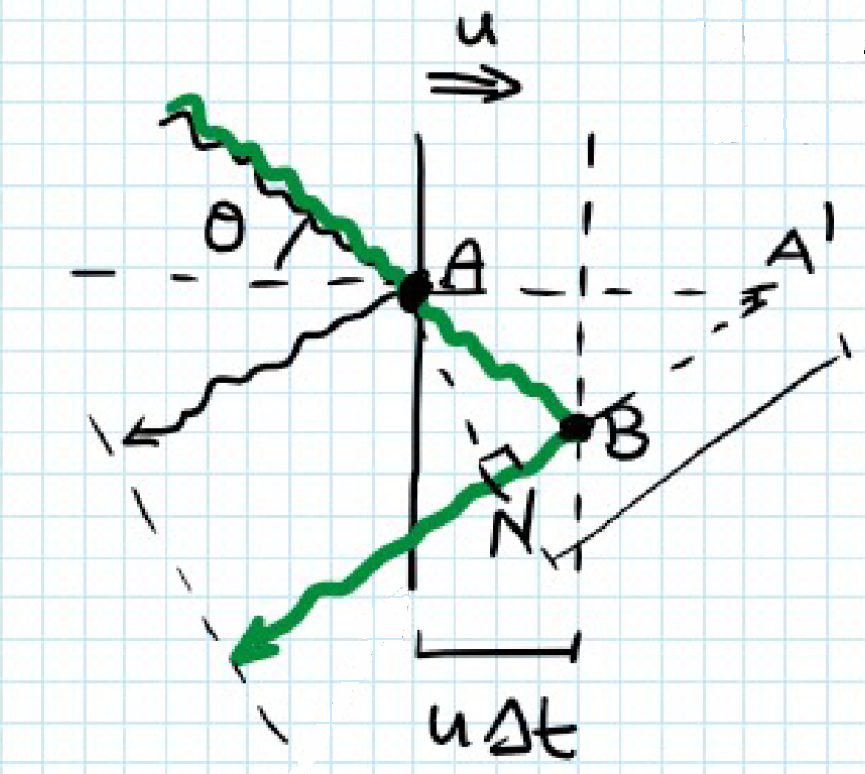
\includegraphics[width=4.5cm]{images/movimento_specchio.png}
\end{figure}\newpage

\noindent
Il tratto che il secondo raggio compie in pi\`u \`e 
\[AB+BN=A'B+BN=A'N=AA'\cos \theta=2u\Delta t \cos \theta.\]
Scegliamo ora $\Delta t=T=\la/c$ periodo dell'onda elettromagnetica. Per definizione la distanza $AB+BN$ in questo caso \`e la variazione di lunghezza d'onda
\[\Delta \la=2\frac {u\la} c\cos \theta.\]
\begin{figure}[!htb]
    \centering
    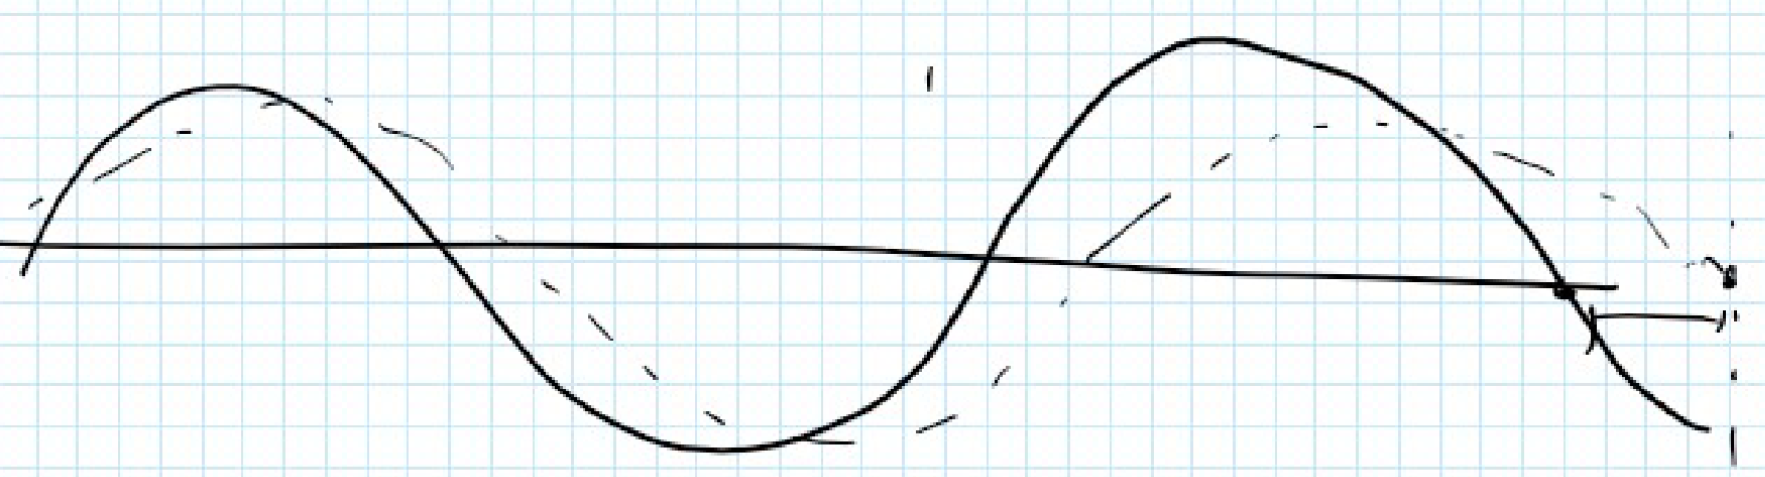
\includegraphics[width=9cm]{images/cambiamento_lunghezza_onda.png}
    \caption{La lunghezza d'onda cambia in modo tale che $\vec E$ sia nullo al bordo, come accade per ogni conduttore.}
\end{figure}

\noindent Tornando alla sfera, poich\'e stiamo considerando trasformazioni adiabatiche, $u/c\ll 1$ e quindi possiamo ipotizzare che nella differenza di tempo appena considerata $\theta$ resti costante e che vicino all'urto valga l'approssimazione piana vista sopra.

\begin{figure}[!htb]
    \centering
    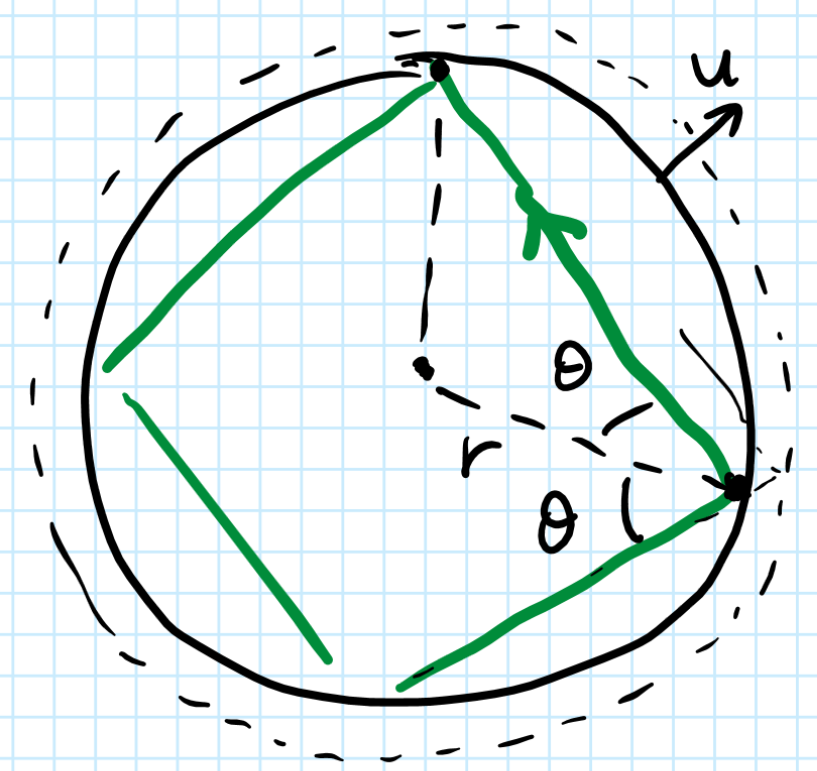
\includegraphics[width=4cm]{images/riflessione_interna_a_sfera.png}
\end{figure}

\noindent
Tra una riflessione e l'altra passa un tempo
\[\frac{2r\cos\theta}c,\]
quindi in un tempo $\Delta t$ avvengono
\[\frac{c\Delta t}{2r\cos\theta}\]
riflessioni.

\noindent
Questo mostra che la variazione di lunghezza d'onda dentro la sfera \`e $2\la\frac uc\cos \theta$ ad ogni riflessione, cio\`e
\[\Delta \la=2\la\frac uc\cos \theta\frac{c\Delta t}{2r\cos \theta}=\frac{\la u\Delta t}r,\]
dunque $\frac{\Delta \la}\la=\frac{u\Delta t}t=\frac{\Delta r }r$, cio\`e $\la\propto r$.\bigskip

\noindent Concludiamo con la seguente catena di proporzionalit\`a
\[\nu\propto \frac1\la\propto \frac1r\propto T.\]
\end{proof}
\begin{remark}
In particolare anche la frequenza a cui abbiamo emissione massima si sposta come $\nu\propto T$. Sperimentalmente
\[\la_{max}=\frac{2.9\mathrm{mm}}{T},\]
dove la temperatura \`e considerata in gradi Kelvin.
\end{remark}

\begin{remark}
Per il sole $\la_{max}(\text{Sole})\sim 502\mathrm{nm}$, cio\`e $T\sim 5800\mathrm{K}$. Potrebbe sembrare una temperatura bassa ma la radiazione di corpo nero viene dalla superficie del sole, quindi la parte pi\`u fredda.
\end{remark}

\begin{proposition}[Vincolo di Wien]\label{VincoloWien}
La dipendenza tra densit\`a di energia e frequenza ha la seguente forma, detta \textbf{vincolo di Wien}
\[\dd \nu w=\nu^3 g(\nu/T).\]
\end{proposition}
\begin{proof}
Consideriamo una certa energia infinitesima a temperatura $T_1$
\[\dd \la w(\la_1)d\la_1.\]
Se ora ci spostiamo alla temperatura $T_2$, questa energia si sposta ad un'altra frequenza $\la_2$. Osserviamo per\`o che, sapendo come si comporta tutto l'integrale ($M\propto T^4$) si ha
\[\frac{\dd \la w(\la_1)d\la_1}{\dd \la w(\la_2)d\la_2}=\frac{T^4_1}{T^4_2}.\]
Poich\'e $\la T$ \`e costante, $\la_1T_1=\la_2T_2$, cio\`e $\dd{\la_2}{\la_1}=\frac{T_2}{T_1}$. Sostituendo\footnote{Slogan: l'integrale va come $T^4$ ma l'integrando va come $T^5$.}
\[\frac1{T_1^5}\dd \la w(\la_1)=\frac1{T_2^5}\dd \la w(\la_2),\]
da cui per lo stesso motivo
\[\la^5\dd \la w=\text{cost.}=f(\la T)\]
per una qualche funzione $f$. Cambiando variabile
\[\dd \nu wd\nu=\nu^3d\nu g(\nu/T)\coimplies \dd \nu w=\nu^3 g(\nu/T).\]
\end{proof}

\noindent
Guardando i dati sperimentali sembrerebbe $g(x)\sim e^{-Bx}$, quindi Wien congettura una legge della forma
\[\dd \nu w=A\nu^3e^{-B\nu/T}\]
detta \textbf{legge di Wien}.




\subsection{Formula di Rayleigh-Jeans}
Scegliamo una scatola cubica con onde di luce dentro e con pareti interne perfettamente riflettenti. Sia $L$ la lunghezza dello spigolo.

\begin{figure}[!htb]
    \centering
    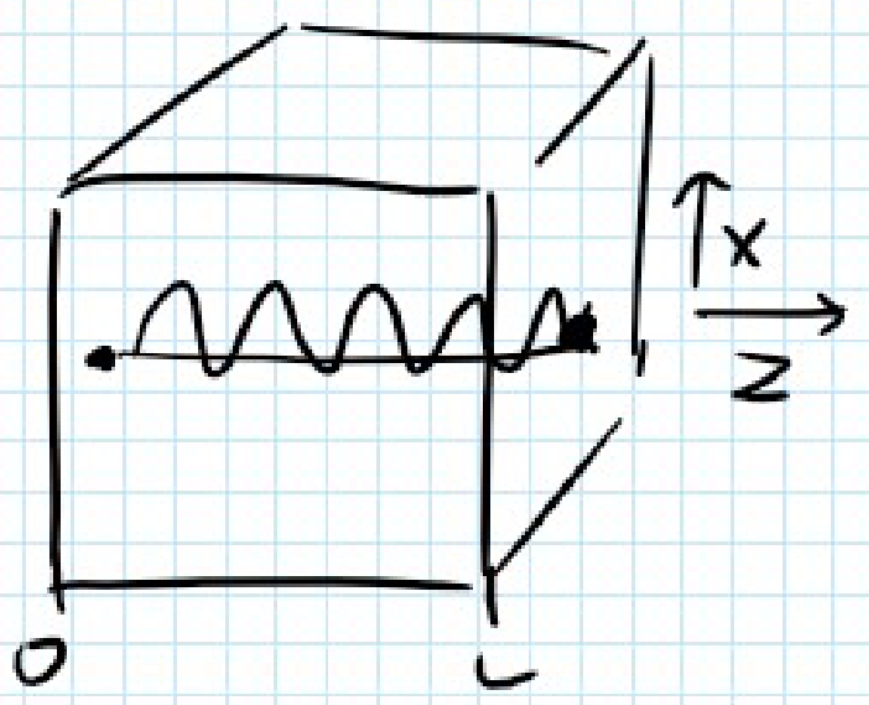
\includegraphics[width=3cm]{images/raggio_dentro_scatola.png}
\end{figure}


\noindent
Ricordiamo che
\[\pps[2]x{E_x}=\frac1{c^2}\pps[2]t{E_x}\]
e che $E_x$ vale $0$ per $x=0$ e $x=L$ (condizioni analoghe valgono per le altre direzioni). Dunque
\[\abs{\vec E}=E_0\sin\pa{n_x\frac{\pi x}L}\sin\pa{n_y\frac{\pi y}L}\sin\pa{n_z\frac{\pi z}L}\]
con $n_x,n_y$ e $n_z$ numeri naturali. Osserviamo che per sottisfare l'equazione dell'onda
\[n_x^2+n_y^2+n_z^2=\frac{4L^2}{\la^4}.\]
Cerchiamo di calcolare il numero possibile di terne. Questo numero intuitivamente corrisponde al numero possibile di onde luminose nella scatola e quindi alla densit\`a di energia.

\begin{figure}[!htb]
    \centering
    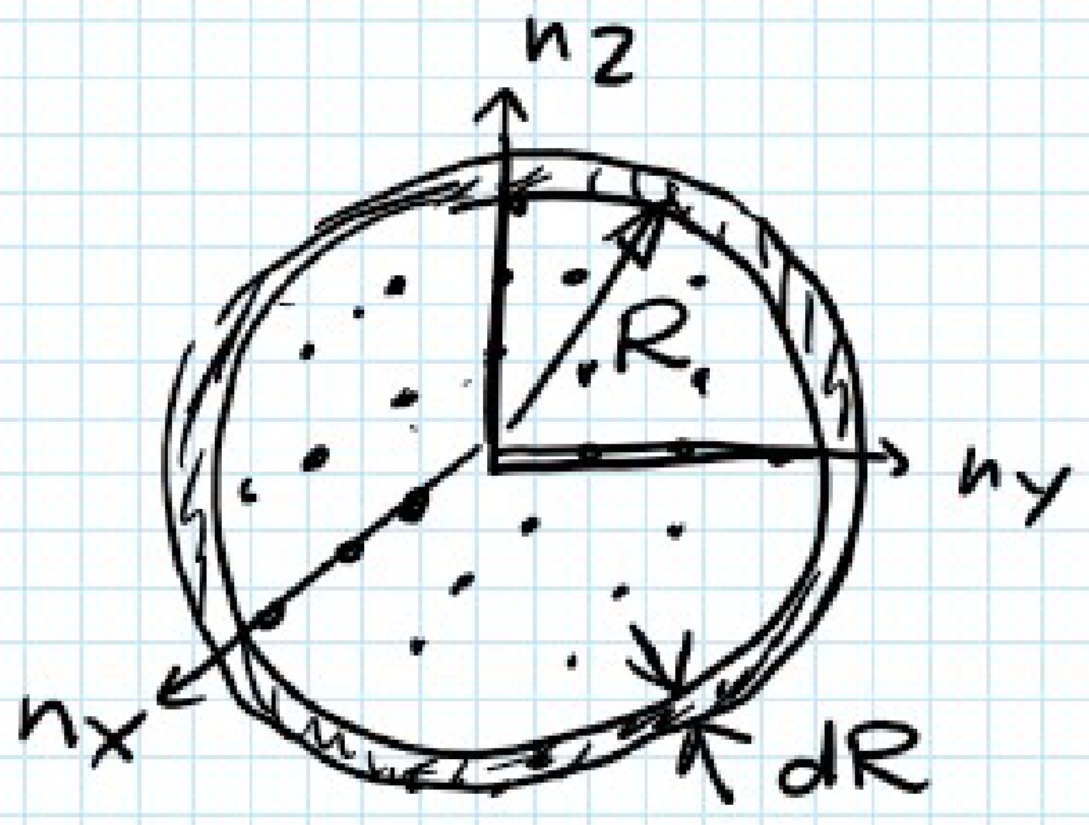
\includegraphics[width=4cm]{images/guscio_sferico.png}
\end{figure}

\noindent
Consideriamo una sfera di raggio $2L/\la$ e cerchiamo i punti del lattice $\Z^3\subseteq \R^3$ vicini alla sfera. Ci aspettiamo un numero di soluzioni $N$ che si comporta come
\[dN=2\frac18 4\pi \pa{\frac{2L}\la}^2 d\pa{\frac{2L}\la}=\frac{8\pi L^3}{\la^4}d\la,\] 
dove il fattore $1/8$ deriva dal fatto che non vogliamo contare come distinte soluzioni che differiscono solo per dei segni e il fattore $2$ serve per tenere conto delle polarizzazioni (in una stessa direzione abbiamo due polarizzazioni indipendenti).\bigskip

\noindent
Ricordando che $V=L^3$ si ha
\[\frac1V\dd \la N=\frac{8\pi}{\la^4}.\]
Cambiando variabile e sfruttando la definizione di $w$ troviamo
\[\boxed{\dd \nu w=\frac{8\pi \nu^2}{c^3}E_{\text{una soluzione}}}\]
\bigskip

\noindent
Lavorando in approssimazione classica $E_{\text{una soluzione}}=k_bT$, cio\`e
\[\dd \nu w=\frac{8\pi \nu^2}{c^3}k_b T.\]
Questa \`e la \textbf{formula di Rayleigh-Jeans}\bigskip

\noindent
Osserviamo per\`o che questa formula non pu\`o funzionare perch\'e per temperature fissate troviamo qualcosa che va come $\nu^2$, che quindi ha integrale infinito in $\nu$, assurdo.

\begin{figure}[!htb]
    \centering
    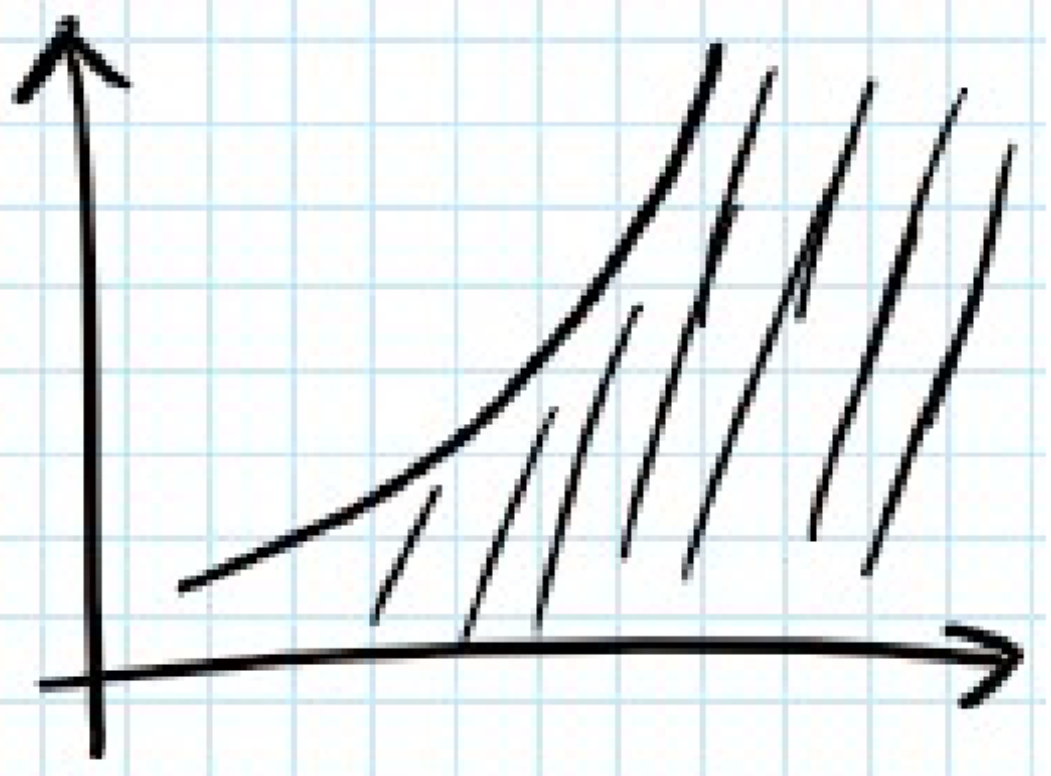
\includegraphics[width=3.5cm]{images/divergenza_problema_corpo_nero}
\end{figure}


\noindent
Questo risultato continua a presentarsi facendo conti classici. Questo \`e detto il \textbf{problema del corpo nero}.

\begin{remark}
La formula di Rayleigh \`e una buona approssimazione per frequenze basse.
\end{remark}


\section{La soluzione di Planck}
Proviamo a rifare questo conto e cerchiamo cosa pu\`o essere andato storto rispetto ai dati sperimentali.\\
La termodinamica \`e intoccabile, quindi
\[\dd \nu w=\frac{8\pi \nu^2}{c^3} E_{\text{una soluzione}}\]
continua a valere.
\begin{itemize}
\item Per alte frequenze sappiamo che
\[\dd \nu w\sim A\nu^3 e^{-B\nu/T},\]
quindi l'energia di una soluzione in questo regime deve avere la forma
\[E=A\nu \frac{c^3}{8\pi} e^{-B\nu/T}\implies \frac{-B\nu}T=\log\pa{\frac{8\pi E}{A\nu c^3}}.\]
Per la termodinamica
\[\ppb USV=\frac1T,\]
quindi
\[\rbar{\dd ES}_V=-\frac1{B\nu}\log\pa{\frac{8\pi E}{A\nu c^3}}\implies \rbar{\dds[2] ES}_V\propto -\frac 1E.\]
\item Per basse frequenze invece notiamo sperimentalmente che la formula di Rayleigh sembra funzionare, cio\`e $E\sim k_bT$, cio\`e per basse frequenze
\[\dd ES=\frac1T\propto\frac1E\implies \rbar{\dds[2] ES}_V\propto -\frac 1E.\]
\end{itemize}
Poniamo allora
\[\dds[2]ES=\frac{-a}{E(b+E)}.\]
Se $E\ll b$ allora questa espressione va come $-1/E$, mentre per alte frequenze va come $-1/E^2$. Integrando segue che
\[E=\frac b{e^{b/(aT)}-1},\]
quindi Planck suppone
\[\dd \nu w=\pa{\frac{8\pi \nu^2}{c^3}}\frac b{e^{b/(aT)}-1}.\]
La formula rispetta il vincolo di Wien se $b\propto \nu$.\bigskip

\noindent
Classicamente\footnote{la densit\`a di probabilit\`a \`e quella ricavata in \ref{EnergiaInternaCostante}}
\[\ps{E}=\frac{\int_0^\infty Ee^{-E/kT}dE}{\int_0^\infty e^{-E/kT}dE}=k_bT,\]
ma noi non vogliamo $k_bT$, vogliamo ritrovare la formula che abbiamo ipotizzato. Supponiamo allora 
\[E_{\text{una soluzione}}=n\e\]
dove $n$ \`e un numero naturale.
\[\ps{E}=\frac{\sum_{n\in\N} n\e e^{-n\e/(k_bT)}}{\sum_{n\in\N}e^{-n\e/(k_bT)}}=\frac \e{e^{\e/(k_bT)}-1}\]
quindi se $\e\propto \nu$ ritroviamo una funzione della forma voluta

\begin{definition}[Costante di Planck]
La \textbf{costante di Planck} $h$ \`e la costante di proporzionalit\`a
\[\e= h\nu,\quad h=6.6\cdot 10^{-34}\ \mathrm{Js}.\]
\end{definition}
\noindent
Sostituendo troviamo la \textbf{distribuzione di Planck}.
\[\boxed{\dd \nu w=\frac{8\pi \nu^3 h}{c^3}\frac1{e^{\frac{h\nu}{k_bT}}-1}}\]


\section{Altri fenomeni}
\subsection{Effetto fotoelettrico}
Consideriamo un pezzo di metallo. Se esso viene colpito da delle onde elettromagnetiche, vengono strappati degli elettroni.\\
Se la luce diventa pi\`u intensa vengono strappati pi\`u eletroni ma non aumenta mai la loro energia. Invece se viene aumentata la frequenza gli elettroni aumentano di energia.\bigskip

\noindent
La spiegazione (Einstein) \`e che la luce viene in pacchetti di energia, detti fotoni. Ogni singolo fotone pu\`o liberare un elettrone, ma l'energia che l'elettrone acquista dipende solo dall'energia del singolo fotone che l'ha colpito.

\subsection{Effetto Compton}
La luce riflessa cambia di frequenza a seconda dell'angolo
\[\nu'=\frac{\nu}{1+\frac{h\nu}{mc^2}(1-\cos\theta)}\]
Se uno fa il conto (Compton), la formula \`e esattamente quella che si ricava considerando un urto dato da una particella di massa nulla secondo la relativit\`a.

\subsection{Spettri atomici}
Diversi atomi emmettono alcune frequenze di radiazione e non altri.\\
Dopo molto tempo Bohr ipotizza che per certi atomi, gli elettroni possono girare attorno al nucleo solo ad alcune frequenze. La differenza tra l'energia alle varie frequenze corrisponde all'energia della luce emessa, che quindi noi misuriamo nelle strisce degli spettri atomici.

\begin{figure}[!htb]
    \centering
    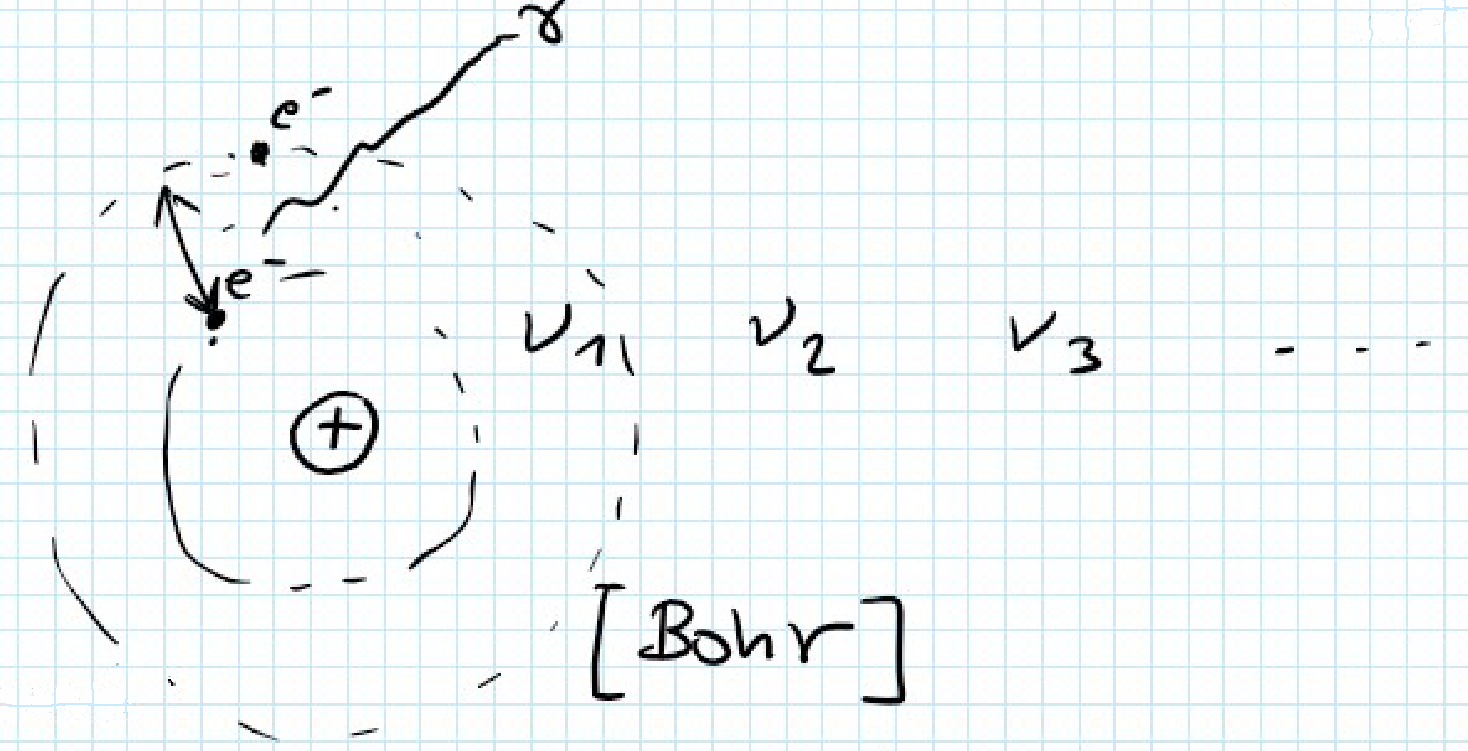
\includegraphics[width=8cm]{images/diverse_frequenze.png}
\end{figure}



